\section{匀速圆周运动}\label{sec:01.10}

    一般情况角速率$\omega$是随$t$变化的,这时质点的速度的大小也
随$t$变化。以下讨论$\omega$不随$t$变化的特殊情况,即匀速圆周运动。
由式\eqref{eqn:01.09.03},这时质点的速率也不变化。质点绕圈周一圈走过的
路程是$2\pi r$。如果走一圈所用时间为$T$,则质点的速率是
\begin{equation}\label{eqn:01.10.01}
    v=\frac{2 \pi r}{T}
\end{equation}
T为周期,比较式\eqref{eqn:01.10.01}、\eqref{eqn:01.09.03},得到:
\begin{equation}\label{eqn:01.10.02}
    \omega=\frac{2 \pi}{T}, ~ T=\frac{2 \pi}{\omega}
\end{equation}
这也就是说,周期$T$等于质点转过$2\pi$角度所需要的时间。

    对于匀速圆周运动,$\vec{v}$的大小不变,而$\vec{v}$的方向时时在变,因
而它的加速度并不为零。由于速度方向总是垂直于矢量$\vec{r}$的,所
以在$t$到$t+\Delta t$间隔中,倘使$\vec{r}$转过角度$\Delta\varphi$,
则$\vec{v}$也就转过了$\Delta\varphi$。由于
$|\vec{v}(t)|=|\vec{v}(t+\Delta t)|=v$,由图\ref{fig:01.22}~的等腰三角形,得
\begin{equation*}
    \begin{aligned}
        |\vec{v}(t+\Delta t)-\vec{v}(t)| &=2 v \sin \frac{\Delta \varphi}{2} \\
        & \approx 2 v\frac{\Delta \varphi}{2}=v \Delta \varphi
    \end{aligned}
\end{equation*}

\begin{figure}[!h]
    \small\centering
    \begin{minipage}[b]{14em}
        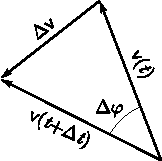
\includegraphics{figure/fig01.22}
        \vspace{1em}
        \caption{匀速圆周运动的加速度}
        \label{fig:01.22}
    \end{minipage}
    \begin{minipage}[b]{14em}
        \centering
        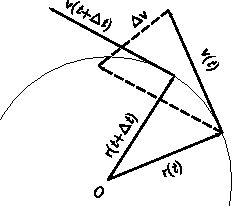
\includegraphics{figure/fig01.23}
        \caption{加速度的方向}
        \label{fig:01.23}
    \end{minipage}
\end{figure}
\noindent 将此式代入式\eqref{eqn:01.08.03},得
\begin{equation}\label{eqn:01.10.03}
    \begin{aligned}
        a & \equiv|\vec{a}|=\lim _{\Delta \rightarrow 0} \frac{|\vec{v}(t+\Delta t)-\vec{v}(t)|}{\Delta t} \\
        &=v\lim_{\boldsymbol{\alpha} \rightarrow 0} \frac{|\Delta \varphi|}{\Delta t}=v \omega=r \omega^{2}=\frac{v^{2}}{r}
    \end{aligned}
\end{equation}\vspace{0.5em}
上式推导中利用了式\eqref{eqn:01.09.02},\eqref{eqn:01.09.03}。因为$v$或$\omega$都不随$t$变,
所以匀速圆周运动的加速度的大小也不随$t$变,但它的方向是时
时变化的。根据图\ref{fig:01.23},当$\Delta t\rightarrow 0$时,
$\vec{v}(t+dt)-\vec{v}(t)=\Delta\vec{v}$的方
向趋于与$\vec{v}(t)$相垂直,并指向圆心。这样,匀速圆周运动的加速
度的大小由式\eqref{eqn:01.10.03}给出,而其方向总是指向圆心的。根据这
种方向上的特点,称这个加速度为向心加速度。

速度、角速度和加速度都是矢量,我们可把式\eqref{eqn:01.10.03}扩充
为矢量关系式:
\clearpage
~\vspace{-1.5em}
\begin{equation}\label{eqn:01.10.04}
    \vec{a}=\omega\times \vec{v}
\end{equation}
它的正确性也留给读者自己去证明。